% ============================================================================
\section{Foundation audio models}
% ============================================================================

% --- Source: Chen et al.\ VALL-E (Works cited 10); TTS Lecture Material Generation Request ---
\begin{frame}{VALL-E: zero-shot TTS}
  \begin{itemize}
    \item VALL-E changes the TTS pipeline to phoneme $\rightarrow$ discrete code $\rightarrow$ waveform, instead of phoneme $\rightarrow$ mel-spectrogram $\rightarrow$ waveform.
    \item The system takes as input a text prompt and a sample of the target voice, tokenizes both (using BPE for text and an audio codec for the speech), and uses a language model to generate discrete audio tokens for the text, matching the target speaker.
    \item VALL-E can do zero-shot TTS, speech editing, and content creation with other generative AI models like GPT-3.
  \end{itemize}
  \centering
  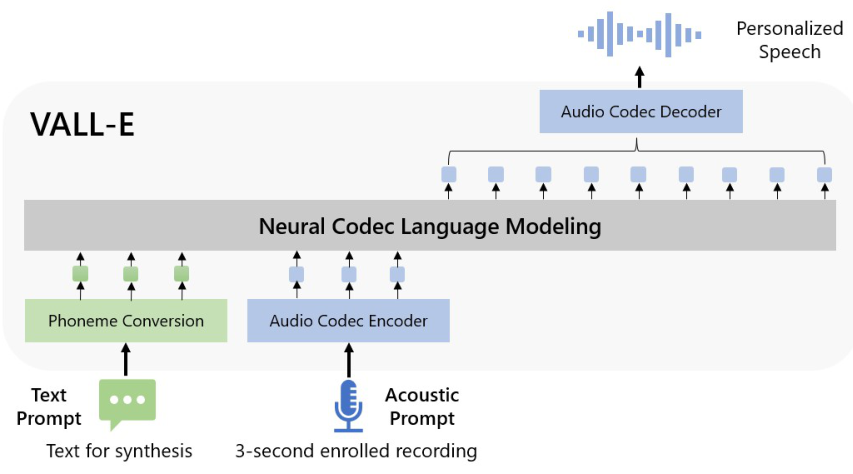
\includegraphics[width=0.92\textwidth,height=0.46\textheight,keepaspectratio]{assets/New-Lecture-TTS/valle_overview_fig1.png}
  \slideimgsource{Wang et al., ``VALL-E: Neural Codec Language Models are Zero-Shot Text to Speech Synthesizers,'' Fig.~1; \href{https://arxiv.org/abs/2301.02111}{arXiv:2301.02111} (cropped).}
\end{frame}

\begin{frame}{VALL-E: comparison with other cascaded TTS systems}
  \centering
  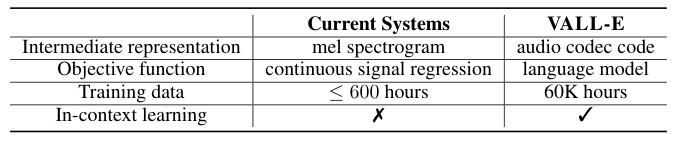
\includegraphics[width=0.92\textwidth,height=0.44\textheight,keepaspectratio]{assets/New-Lecture-TTS/valle_page2.png}
  \slideimgsource{Chen et al., VALL-E, Fig.~2: comparison with other cascaded TTS systems.}
\end{frame}

\begin{frame}{VALL-E: Limitations}
  \begin{itemize}\footnotesize
    \item \textbf{Data requirements:} VALL-E requires large amounts of high-quality paired text and audio data for effective training.
    \item \textbf{Speaker similarity:} The system relies on a reference sample; quality of voice cloning can degrade for voices and accents underrepresented in training.
    \item \textbf{Codec/token bottlenecks:} Using discrete audio tokens (from speech codebooks) may cause artifacts or limit audio fidelity compared to raw waveform modeling.
    \item \textbf{Generalization:} Performance may drop for out-of-distribution prompts or novel voice/text combinations not seen in training.
    \item \textbf{Ethical concerns:} Zero-shot voice synthesis can enable impersonation and raises privacy and misuse risks.
  \end{itemize}
\end{frame}

\begin{frame}{Voicebox: GPT-like generalist for audio}
  \begin{itemize}\footnotesize
    \item Non-autoregressive flow-matching model trained to fill in missing speech given context audio and full transcript.
    \begin{itemize}
      \item Style comes from audio context; content comes from text.
    \end{itemize}    
    \item One model handles zero-shot TTS, denoising, editing, style transfer, and diverse sampling via in-context learning.
    \item Gains over VALL-E on intelligibility and speaker similarity, up to \textbf{20$\times$} faster generation.
  \end{itemize}
\end{frame}

\begin{frame}{Voicebox: Approach}
  \begin{itemize}\footnotesize
    \item Training: learn $p(x_{\text{masked}} \mid y, x_{\text{context}})$---fill a random masked span using transcript $y$ and unmasked audio.
    \item Two modules: an audio model (80-dim log-mel frames, Transformer) and a duration model.
    \item \textbf{Inference:} Sample random noise, which is then shaped into meaningful speech representations (mel spectrogram frames) by solving a continuous flow ordinary differential equation (ODE) conditioned on both the transcript and audio context. After obtaining the predicted mel spectrogram, a neural vocoder is used to convert these mel frames into audible waveform speech, thus completing the synthesis pipeline.
  \end{itemize}
  \centering
  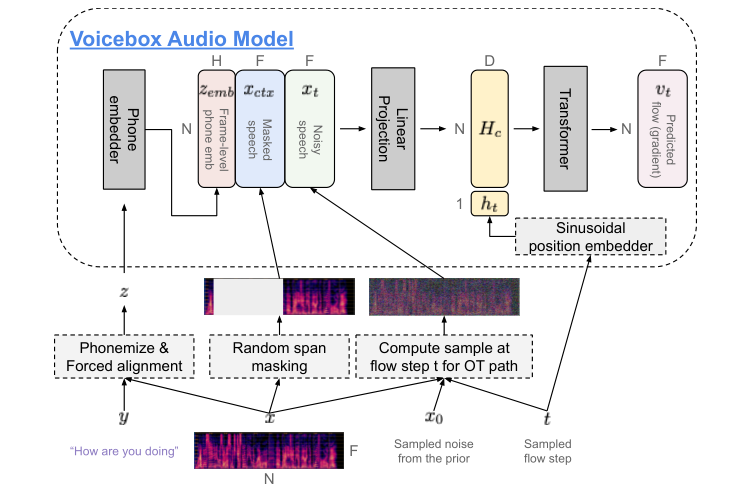
\includegraphics[width=0.95\textwidth,height=0.38\textheight,keepaspectratio]{assets/New-Lecture-TTS/voicebox_fig2_audio_model.png}
  \slideimgsource{Le et al., Voicebox, Fig.~1: task generalization through in-context learning; \href{https://arxiv.org/abs/2306.15687}{arXiv:2306.15687}.}
\end{frame}

\begin{frame}{Voicebox: limitations}
  \begin{itemize}\footnotesize
    \item \textbf{Read speech domain:} trained mainly on audiobooks; may not transfer well to casual conversation (laughter, back-channels).
    \item \textbf{Front-end dependency:} needs a phonemizer and forced aligner; word-based phonemizers miss context-sensitive pronunciation.
    \item \textbf{Limited control:} can transfer overall style from prompts, but cannot separately pick voice from one clip and emotion from another.
    \item \textbf{Bias risk:} performance can drop for underrepresented accents unless training data stays diverse.
    \item \textbf{Misuse:} high-quality cloning raises deepfake concerns---authors release a strong synthetic-speech \textbf{classifier} as a mitigation.
  \end{itemize}
\end{frame}

% --- Source: TTS Lecture Material Generation Request (model comparison table) ---
\begin{frame}{Architectures at a glance}
  \footnotesize
  \begin{tabular}{@{}llll@{}}
    \hline
    \textbf{Model} & \textbf{Paradigm} & \textbf{Representation} & \textbf{Highlight} \\
    \hline
    Tacotron~2 & AR seq2seq & Mel & Strong naturalness \\
    FastSpeech~2 & NAR Transformer & Mel & Fast; explicit prosody \\
    Glow-TTS & Flow + MAS & Mel & Hard alignments \\
    VALL-E & Codec LM & Discrete codes & Zero-shot cloning \\
    Voicebox & Flow matching & Continuous audio & Infilling / editing \\
    \hline
  \end{tabular}
\end{frame}
